\documentclass[11pt,a4paper]{article}
\usepackage[T1]{fontenc}
\usepackage[utf8]{inputenc}
\usepackage{mathptmx}
\usepackage[margin=24mm]{geometry}
\usepackage{microtype}
\usepackage{amsmath}
\usepackage{booktabs,array,tabularx}
\usepackage{tikz}
\usetikzlibrary{arrows.meta,positioning,calc,fit,patterns}
\usepackage{pgfplots}
\pgfplotsset{compat=1.18}
\usepackage{caption}
\usepackage{hyperref}
\hypersetup{hidelinks,pdftitle={PatchTST for Parkinson's Speech Classification: A Plain-English Technical Report},pdfauthor={Arannamoy Mondal},pdfsubject={Single-model v2.0 pipeline, speaker-level OOF evaluation and leakage audit}}
\setlength{\parindent}{0pt}
\setlength{\parskip}{6pt}
\setlength{\emergencystretch}{2em}
\makeatletter
\def\@listi{\leftmargin\leftmargini\parsep 0pt\topsep 4pt\itemsep 2pt}
\let\@listI\@listi
\newcommand{\tableinput}[1]{\@@input #1 }
\makeatother
\renewcommand{\arraystretch}{1.22}
\captionsetup{font=small,labelfont=bf,justification=raggedright,singlelinecheck=false,hypcap=false}
\pagestyle{plain}
\newcolumntype{L}[1]{>{\raggedright\arraybackslash}p{#1}}
\newcolumntype{Y}{>{\raggedright\arraybackslash}X}
\newcommand{\key}[1]{\textbf{#1}}
\newcommand{\sourcepath}[1]{{\small\path{#1}}}
\newcommand{\rulebox}[1]{\par\smallskip\noindent\fbox{\parbox{\dimexpr\linewidth-2\fboxsep-2\fboxrule\relax}{#1}}\par\smallskip}
\newcommand{\diagramcaption}[1]{\captionof{figure}{#1}}
\tikzset{
  box/.style={draw=black,fill=white,rectangle,align=center,inner sep=6pt,font=\small},
  wide/.style={box,text width=11.8cm,minimum height=0.8cm},
  smallbox/.style={box,text width=3.1cm,minimum height=1cm},
  arrow/.style={-{Stealth[length=2mm]},line width=0.6pt,draw=black},
  note/.style={align=left,font=\small},
  every picture/.style={line width=0.5pt}
}

\begin{document}

\begin{center}
{\LARGE\bfseries PatchTST for Parkinson's\\[3pt] Speech Classification\par}
\vspace{8pt}
{\large A Plain-English Technical Report\par}
\vspace{10pt}
Arannamoy Mondal\\
\href{mailto:arannamoymondal13@gmail.com}{arannamoymondal13@gmail.com}\\[5pt]
12 October 2026\quad\textbullet\quad Report 1.0\quad\textbullet\quad Experiment v2.0
\end{center}
\vspace{3pt}\hrule\vspace{8pt}

\section*{Abstract}
This report explains one model from start to finish: a compact PatchTST classifier
that uses speech to distinguish people with Parkinson's disease from elderly
healthy controls. It explains how recordings are checked, how repeat sessions
are linked to the same person, how sound becomes a spectrogram, how the model is
trained, and how many short-window scores become one decision per person.

The main experiment uses 773 recordings from 46 people: 25 patients and 21
controls. Five speaker-disjoint folds keep each test person's recordings out of
the model that predicts that person. The pooled speaker-level results are F1
97.96\%, recall 96.00\%, specificity 100.00\%, precision 100.00\%, and accuracy
97.83\%. There is one missed patient and no false alarms among controls.

The saved results reproduce. However, the recordings also contain strong
group-related acoustic differences, and recording dates are separated by class.
The report therefore explains both the leakage controls that were checked and
the recording-condition problem that remains. These are internal results on
this corpus, not an independent clinical validation.

\section{One question, one model, one input}
The question is simple: \emph{using speech recordings, can this model separate
people labeled with Parkinson's disease from elderly healthy controls in this
dataset?} The recorded diagnosis supplies the training label. The model predicts
that label; it does not create a new medical diagnosis.

\begin{center}
\begin{tabularx}{\linewidth}{@{}L{3.3cm}Y@{}}
\toprule
Model & Corrected, channel-independent PatchTST; experiment v2.0.\\
Input & A 64-band log-mel spectrogram, cut into 400-frame windows.\\
Output & One model score per window, combined into one speaker score.\\
Decision & Score at least 0.5: PD; score below 0.5: elderly control.\\
Evaluation unit & One person, not one recording or one short window.\\
\bottomrule
\end{tabularx}
\end{center}

\key{How to read this report.} Sections 2--7 describe the data and model.
Sections 8--11 explain training, OOF predictions and score averaging.
Sections 12--15 give the results and their limits. Sections 16--17 explain
reproduction and the main terms. Diagrams use black lines, labels and shapes so
they remain readable in a black-and-white printout.

\clearpage
\section{The whole pipeline in one picture}
Read Figure~\ref{fig:full} from top to bottom. A \emph{manifest} is simply a table
with one row for each recording. A \emph{fold} is one group of people held aside
for testing. The same model design is trained separately for each fold.

\begin{center}
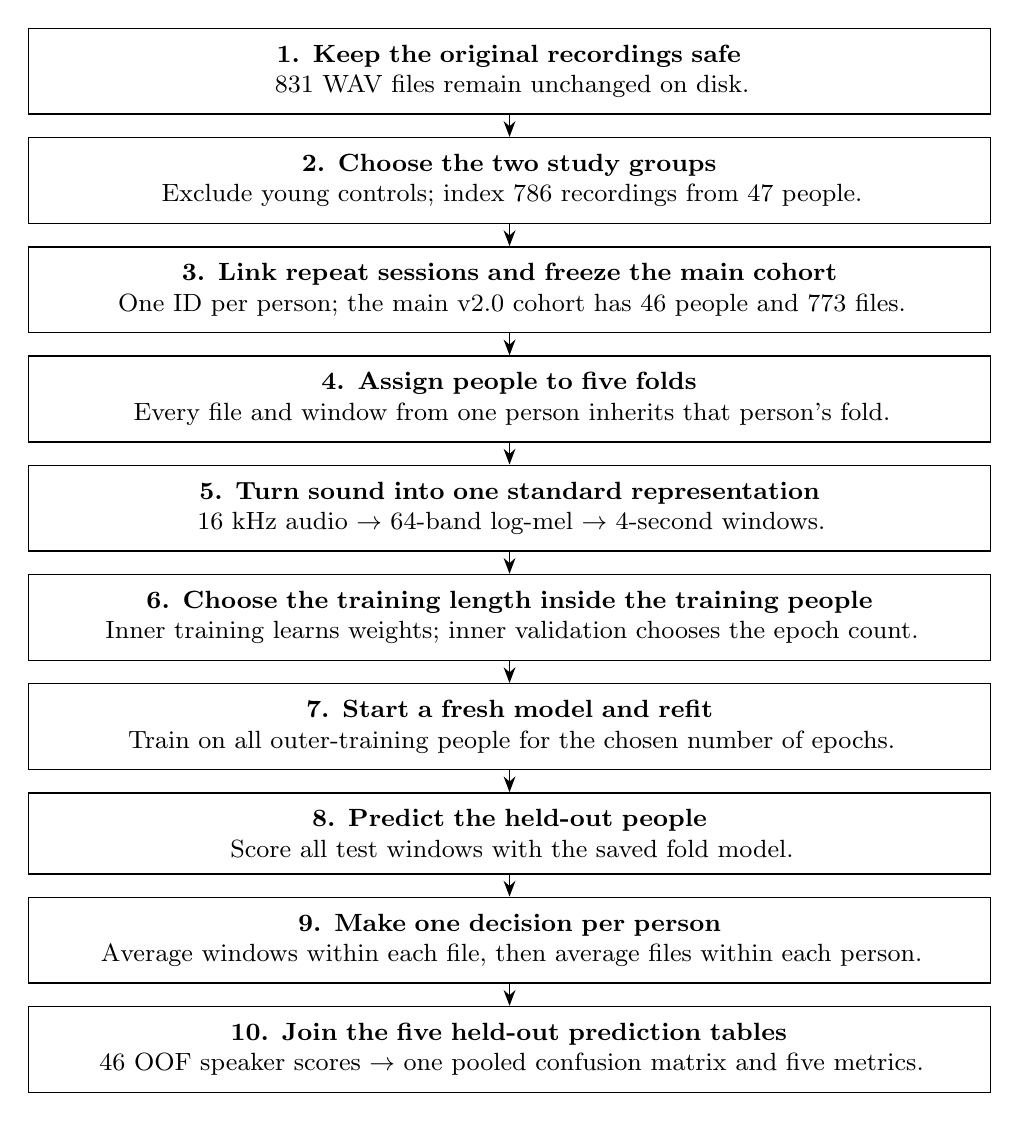
\begin{tikzpicture}[node distance=0.28cm]
\node[wide] (raw) {\textbf{1. Keep the original recordings safe}\\831 WAV files remain unchanged on disk.};
\node[wide,below=of raw] (cohort) {\textbf{2. Choose the two study groups}\\Exclude young controls; index 786 recordings from 47 people.};
\node[wide,below=of cohort] (identity) {\textbf{3. Link repeat sessions and freeze the main cohort}\\One ID per person; the main v2.0 cohort has 46 people and 773 files.};
\node[wide,below=of identity] (split) {\textbf{4. Assign people to five folds}\\Every file and window from one person inherits that person's fold.};
\node[wide,below=of split] (features) {\textbf{5. Turn sound into one standard representation}\\16 kHz audio $\rightarrow$ 64-band log-mel $\rightarrow$ 4-second windows.};
\node[wide,below=of features] (select) {\textbf{6. Choose the training length inside the training people}\\Inner training learns weights; inner validation chooses the epoch count.};
\node[wide,below=of select] (refit) {\textbf{7. Start a fresh model and refit}\\Train on all outer-training people for the chosen number of epochs.};
\node[wide,below=of refit] (predict) {\textbf{8. Predict the held-out people}\\Score all test windows with the saved fold model.};
\node[wide,below=of predict] (average) {\textbf{9. Make one decision per person}\\Average windows within each file, then average files within each person.};
\node[wide,below=of average] (pool) {\textbf{10. Join the five held-out prediction tables}\\46 OOF speaker scores $\rightarrow$ one pooled confusion matrix and five metrics.};
\foreach \a/\b in {raw/cohort,cohort/identity,identity/split,split/features,features/select,select/refit,refit/predict,predict/average,average/pool}
  \draw[arrow] (\a) -- (\b);
\end{tikzpicture}
\diagramcaption{The complete single-model workflow. Steps 6--9 run once for each
held-out fold. OOF means that a person's score comes from the model trained
without that person.}\label{fig:full}
\end{center}

\key{Two kinds of work happen here.} Fixed audio conversion can be cached once
because it learns no statistics from the dataset. Learning weights and choosing
how long to train happen inside each training split. Section~\ref{sec:leakage}
explains why that boundary matters.

\clearpage
\section{Which recordings and people enter the study?}
The source is the Italian Parkinson's Voice and Speech corpus~\cite{dataport},
associated with the VoxTester and speech-intelligibility work~\cite{voxtester,access}.
The folder name ``28 People with Parkinson's disease'' is a folder count, not the
final number of distinct patients. Linking repeat sessions gives 25 patient IDs.

\begin{center}
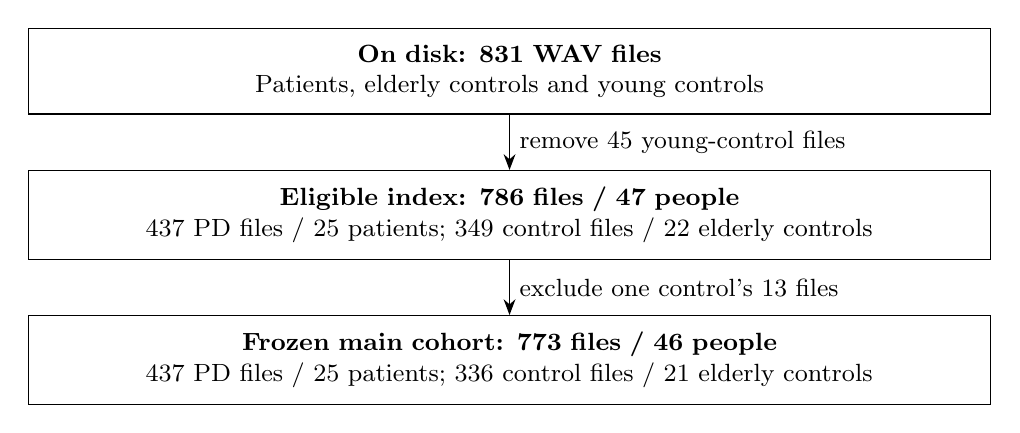
\begin{tikzpicture}[node distance=0.7cm]
\node[wide] (all) {\textbf{On disk: 831 WAV files}\\Patients, elderly controls and young controls};
\node[wide,below=of all] (eligible) {\textbf{Eligible index: 786 files / 47 people}\\437 PD files / 25 patients; 349 control files / 22 elderly controls};
\node[wide,below=of eligible] (main) {\textbf{Frozen main cohort: 773 files / 46 people}\\437 PD files / 25 patients; 336 control files / 21 elderly controls};
\draw[arrow] (all) -- node[right,font=\small] {remove 45 young-control files} (eligible);
\draw[arrow] (eligible) -- node[right,font=\small] {exclude one control's 13 files} (main);
\end{tikzpicture}
\diagramcaption{The counts at each stage. Excluded recordings remain on disk;
exclusion means that their rows do not enter the experiment.}
\end{center}

\subsection*{Why exclude young controls?}
The 15 young controls are aged 19--29. Including them could reward a model for
detecting age rather than disease. This study uses elderly controls as the
comparison group. That reduces an obvious age difference, but does not guarantee
that every age or recruitment effect is removed.

\subsection*{Why does the main result contain 46 rather than 47 people?}
The completed v2.0 experiment froze a common, task-available cohort for the
original project comparison. One elderly control, Vitantonio D, has no B1/B2
passage recordings, so that cohort excluded him. This report keeps that exact
46-person cohort to match the saved result. PatchTST itself does not require
every person to have a passage; this exclusion is an evaluation-design choice.

\begin{center}
\begin{tabularx}{\linewidth}{@{}L{3.0cm}L{4.8cm}rY@{}}
\toprule
Speech task & Meaning in everyday words & Files & Codes\\
\midrule
Passages & Read a longer piece of text & 94 & B1, B2\\
Repeated syllables & Repeat short sounds such as /pa/ and /ta/ & 98 & D1, D2\\
Vowels & Hold a vowel sound & 485 & VA1--VU2\\
Words & Read a word list & 49 & PR1\\
Phrases & Read short phrases & 47 & FB1\\
\midrule
Total & All these tasks enter PatchTST & 773 & \\
\bottomrule
\end{tabularx}
\end{center}

\key{Labels.} PD is 1; elderly healthy control is 0. Labels come from the exact
group folder. Searching for the word ``Parkinson'' anywhere in a path would be
wrong because the dataset's root folder also contains that word.

\clearpage
\section{One person must keep one identity}
The same person can have several recordings, several tasks, or more than one
recording session. Those are repeated observations of one person. They must not
be mistaken for different people when training and testing are separated.

\begin{center}
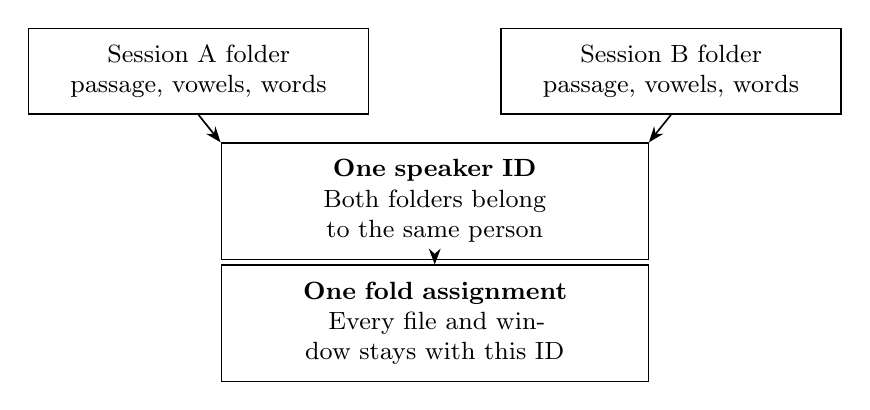
\begin{tikzpicture}
\node[box,text width=3.9cm] (a) at (0,0) {Session A folder\\passage, vowels, words};
\node[box,text width=3.9cm] (b) at (6,0) {Session B folder\\passage, vowels, words};
\node[box,text width=5.0cm] (id) at (3,-1.65) {\textbf{One speaker ID}\\Both folders belong to the same person};
\node[box,text width=5.0cm] (fold) at (3,-3.2) {\textbf{One fold assignment}\\Every file and window stays with this ID};
\draw[arrow] (a.south) -- (id.north west);
\draw[arrow] (b.south) -- (id.north east);
\draw[arrow] (id) -- (fold);
\end{tikzpicture}
\diagramcaption{Repeat sessions are joined before folds are created. The person
is the unit of separation, even when dates, folders or token spellings differ.}
\end{center}

\subsection*{The identity checks used here}
The index reads the task, person token and recording time from each filename.
Known text problems are corrected in the index; the original file is not renamed.
Folders are linked using the same cohort and matching person tokens, with the
documented name/birth-year/sex matches used for known repeat sessions.

\begin{itemize}
\item Vito S with token ending \texttt{46M} is linked across his two sessions.
\item Nicola S and Roberto R are linked despite two spellings of their tokens.
\item The other Vito S, whose token ends in \texttt{47M}, stays a different person.
\item Antonia G has one inconsistent export token. The folder's usual token is
used, and that recording receives a correction flag.
\end{itemize}

These are the project's working identity rules. The audit checks them against
the known corpus records; it does not claim biometric proof of every identity.

\subsection*{A useful file table does not become a model input}
The manifest stores the speaker ID, label, task, original sample rate, duration,
date, fold and cache path. Age, sex and spreadsheet fields help check records.
\key{The network receives only the spectrogram values.} It does not receive a
name, filename, age, sex, recording date, reading-speed score or native sample rate.

A \texttt{sheet\_flag} records a review mark in the source spreadsheet. Four
eligible controls have this flag; three are present in the main cohort. They
remain in the main evaluation. Section~\ref{sec:checks} shows the check that
removes them from scoring.

\rulebox{\textbf{The rule to remember:} a new folder does not mean a new person.
Create the person ID first; then split the people.}

\clearpage
\section{Preprocessing: turning sound into a useful table}
Audio is a long list of sample values. A spectrogram turns that list into a
time-by-frequency description: it shows which frequency ranges carry energy at
each short time step. The model uses the numerical table, not a screenshot.

\begin{center}
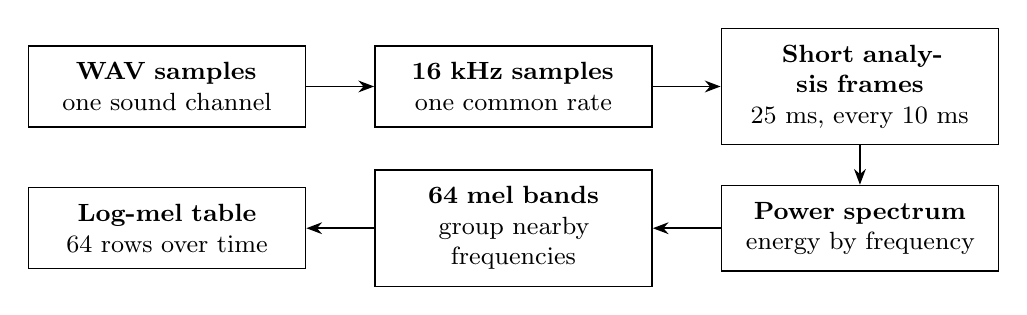
\begin{tikzpicture}
\node[smallbox] (wav) at (0,0) {\textbf{WAV samples}\\one sound channel};
\node[smallbox] (rate) at (4.4,0) {\textbf{16 kHz samples}\\one common rate};
\node[smallbox] (frames) at (8.8,0) {\textbf{Short analysis frames}\\25 ms, every 10 ms};
\node[smallbox] (log) at (0,-1.8) {\textbf{Log-mel table}\\64 rows over time};
\node[smallbox] (mel) at (4.4,-1.8) {\textbf{64 mel bands}\\group nearby frequencies};
\node[smallbox] (power) at (8.8,-1.8) {\textbf{Power spectrum}\\energy by frequency};
\draw[arrow] (wav) -- (rate);
\draw[arrow] (rate) -- (frames);
\draw[arrow] (frames) -- (power);
\draw[arrow] (power) -- (mel);
\draw[arrow] (mel) -- (log);
\end{tikzpicture}
\diagramcaption{Fixed preprocessing applied separately to each recording.
``ms'' means milliseconds; 1,000 milliseconds make one second.}
\end{center}

\subsection*{Read and resample}
The corpus WAVs are mono, 16-bit PCM. They are read as 32-bit floating-point
numbers on a common digital scale. If the original sample rate is 44,100 Hz,
the waveform is resampled to 16,000 Hz using \texttt{soxr\_hq}. Native 16,000-Hz
files are read directly. Resampling changes the number of samples per second;
it does not intentionally make the person speak faster or slower.

\subsection*{Measure frequency energy in short frames}
A 400-sample analysis window covers 25 ms at 16 kHz. The next frame starts 160
samples, or 10 ms, later. A 512-point Fourier transform separates frequency
content. Sixty-four overlapping mel filters combine that energy into bands
spaced more closely at lower frequencies. The implementation uses librosa's
default Hann analysis window and centered-frame convention.

\subsection*{Use the same logarithmic reference for every file}
Power values are converted to decibels using a fixed reference of 1.0 and a
power floor of $10^{-10}$. The floor avoids taking a logarithm of zero.
In simplified form, for a band power $P$,
\[
X=10\log_{10}\!\left(\frac{\max(P,10^{-10})}{1.0}\right).
\]
There is no per-file peak normalization and no per-file maximum as the decibel
reference. Recording-relative decibel clipping is disabled. This keeps digital
level differences visible. A quiet voice can be informative, but gain and
microphone distance can change the same numbers. Digital level is not calibrated
physical voice loudness.

\rulebox{\textbf{Two different windows:} the 25-ms analysis window builds each
spectrogram frame. The 4-second model window later groups 400 frames into one
model input. They do different jobs.}

\clearpage
\section{Windows and patches: three different time scales}
The spectrogram has 64 frequency-band rows and a variable number of time
columns. Roughly 100 columns describe one second. Centering can add a boundary
frame, so full-file frame counts are only approximately duration times 100.

\begin{center}
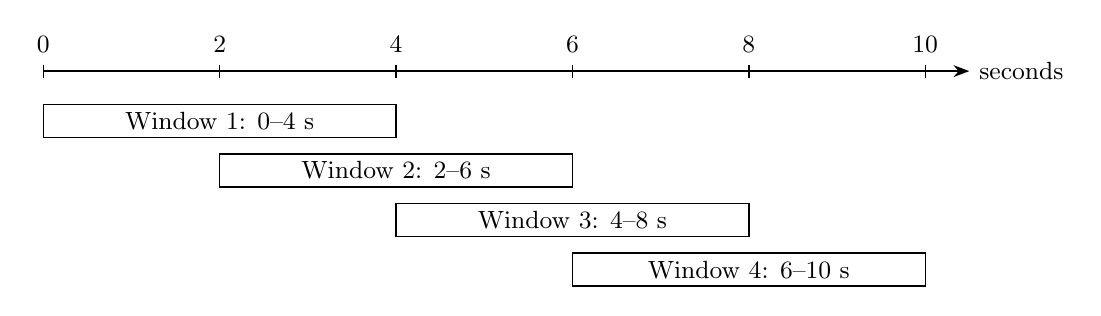
\begin{tikzpicture}[x=1.12cm,y=0.7cm]
\draw[arrow] (0,0) -- (10.5,0) node[right,font=\small] {seconds};
\foreach \x in {0,2,4,6,8,10} {
  \draw (\x,0.12) -- (\x,-0.12);
  \node[font=\small,above] at (\x,0.15) {\x};
}
\draw (0,-0.6) rectangle (4,-1.2);
\node[font=\small] at (2,-0.9) {Window 1: 0--4 s};
\draw (2,-1.5) rectangle (6,-2.1);
\node[font=\small] at (4,-1.8) {Window 2: 2--6 s};
\draw (4,-2.4) rectangle (8,-3.0);
\node[font=\small] at (6,-2.7) {Window 3: 4--8 s};
\draw (6,-3.3) rectangle (10,-3.9);
\node[font=\small] at (8,-3.6) {Window 4: 6--10 s};
\end{tikzpicture}
\diagramcaption{A simple timeline sketch. Four-second windows move forward by
two seconds, so nearby windows share sound. The actual code works in frame
indices and adds a final window when needed to cover the end.}
\end{center}

\begin{center}
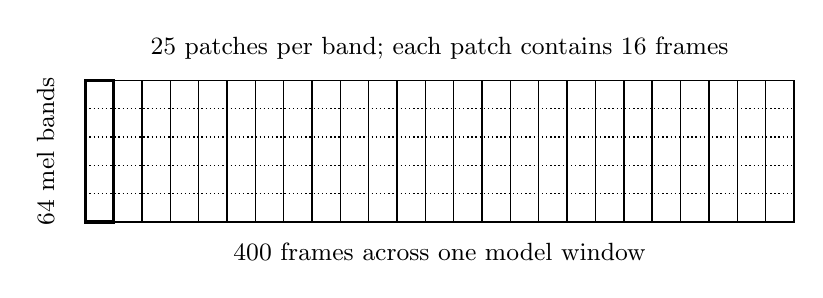
\begin{tikzpicture}[x=0.36cm,y=0.36cm]
\draw (0,0) rectangle (25,5);
\foreach \x in {1,...,24} \draw (\x,0) -- (\x,5);
\foreach \y in {1,...,4} \draw[densely dotted] (0,\y) -- (25,\y);
\draw[line width=1.2pt] (0,0) rectangle (1,5);
\node[font=\small,rotate=90] at (-1.4,2.5) {64 mel bands};
\node[font=\small,below] at (12.5,-0.4) {400 frames across one model window};
\node[font=\small,above] at (12.5,5.4) {25 patches per band; each patch contains 16 frames};
\end{tikzpicture}
\diagramcaption{An input-shape sketch, not a measured spectrogram. Only a few
horizontal guide lines are drawn. The real numerical input has 64 rows.}
\end{center}

\begin{itemize}
\item \key{Model input:} 64 bands $\times$ 400 frames. That is 25,600 numerical
values, not 25,600 separately designed acoustic features.
\item \key{Short files:} if fewer than 400 frames are available, the final frame
is repeated until the window is full. This is called edge padding.
\item \key{Training:} keep at most eight evenly spaced windows from each file.
\item \key{Validation and testing:} keep every window, including final-tail coverage.
\item \key{Inside PatchTST:} split each band into 25 non-overlapping patches of
16 frames. Patch starts are 160 ms apart; analysis frames themselves overlap.
\end{itemize}

\key{Why split people first?} Overlapping windows can contain much of the same
audio. A random window split could place near-identical sound in both training
and testing. In this pipeline, every window follows its person's existing fold.

\clearpage
\section{What the PatchTST model actually does}
PatchTST's original idea is to read short time patches and reuse one encoder
across channels~\cite{patchtst}. Here it is adapted to classification: each mel
band acts as one channel. This is a compact project implementation, not a claim
to have invented PatchTST or reproduced its forecasting benchmark.

\begin{center}
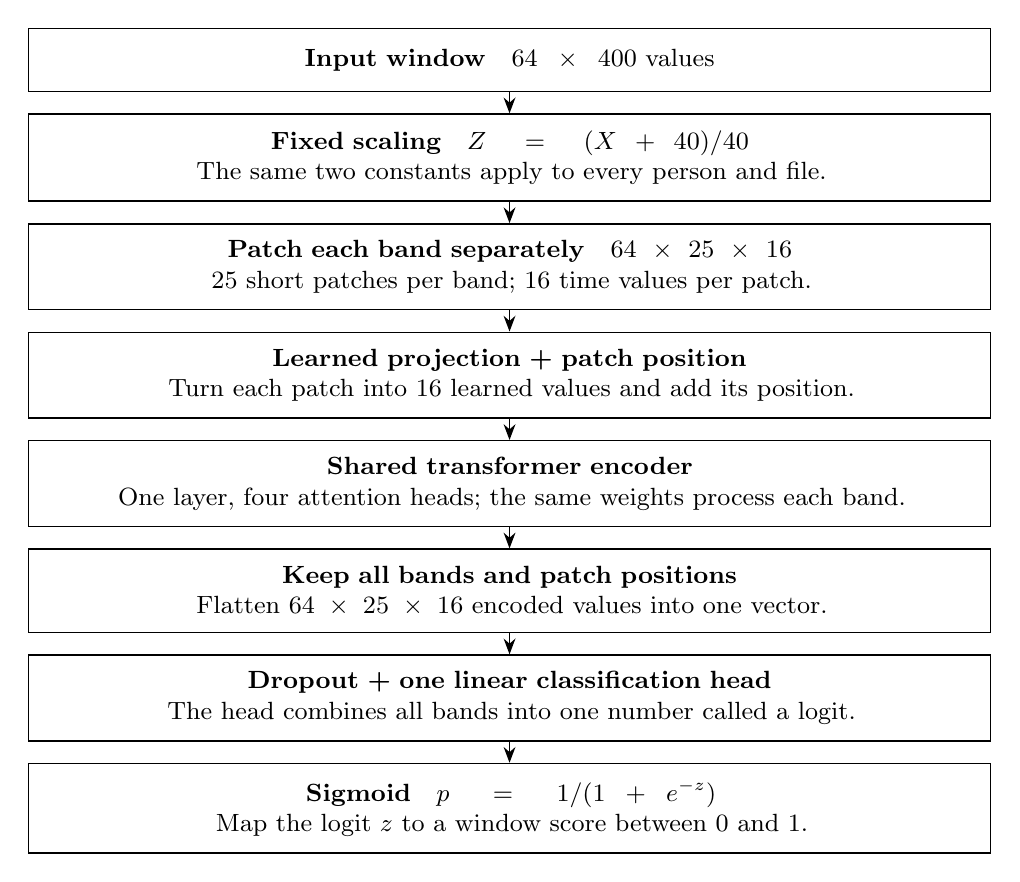
\begin{tikzpicture}[node distance=0.27cm]
\node[wide] (input) {\textbf{Input window}\quad $64\times400$ values};
\node[wide,below=of input] (scale) {\textbf{Fixed scaling}\quad $Z=(X+40)/40$\\The same two constants apply to every person and file.};
\node[wide,below=of scale] (patch) {\textbf{Patch each band separately}\quad $64\times25\times16$\\25 short patches per band; 16 time values per patch.};
\node[wide,below=of patch] (embed) {\textbf{Learned projection + patch position}\\Turn each patch into 16 learned values and add its position.};
\node[wide,below=of embed] (encode) {\textbf{Shared transformer encoder}\\One layer, four attention heads; the same weights process each band.};
\node[wide,below=of encode] (flatten) {\textbf{Keep all bands and patch positions}\\Flatten $64\times25\times16$ encoded values into one vector.};
\node[wide,below=of flatten] (head) {\textbf{Dropout + one linear classification head}\\The head combines all bands into one number called a logit.};
\node[wide,below=of head] (prob) {\textbf{Sigmoid}\quad $p=1/(1+e^{-z})$\\Map the logit $z$ to a window score between 0 and 1.};
\foreach \a/\b in {input/scale,scale/patch,patch/embed,embed/encode,encode/flatten,flatten/head,head/prob}
  \draw[arrow] (\a) -- (\b);
\end{tikzpicture}
\diagramcaption{The single classifier used in this report. Dimensions exclude
the batch size. The model has 29,553 trainable parameters.}
\end{center}

\key{Attention} lets a patch use information from other patches in the same
band. Four heads provide four learned ways of comparing those patches.
The encoder width is 16 and its feed-forward width is 64, with GELU activation.
\key{Channel-independent} means that bands share the encoder's weights and do
not attend across bands there. The final head combines the bands.

Position embeddings allow time order to matter; they do not prove that the
trained decisions need it. The later audit found the main decisions survived
strong changes to within-window temporal detail. A model score is also not a
calibrated estimate of a person's clinical probability of disease.

\clearpage
\section{OOF: how each person receives a held-out score}\label{sec:oof}
\key{OOF means out-of-fold.} First, the 46 people are divided into five groups.
For each group, a separate model is trained using only the other four groups.
That model then predicts the held-out group. The five held-out tables are joined
into one table containing each person exactly once.

\begin{center}
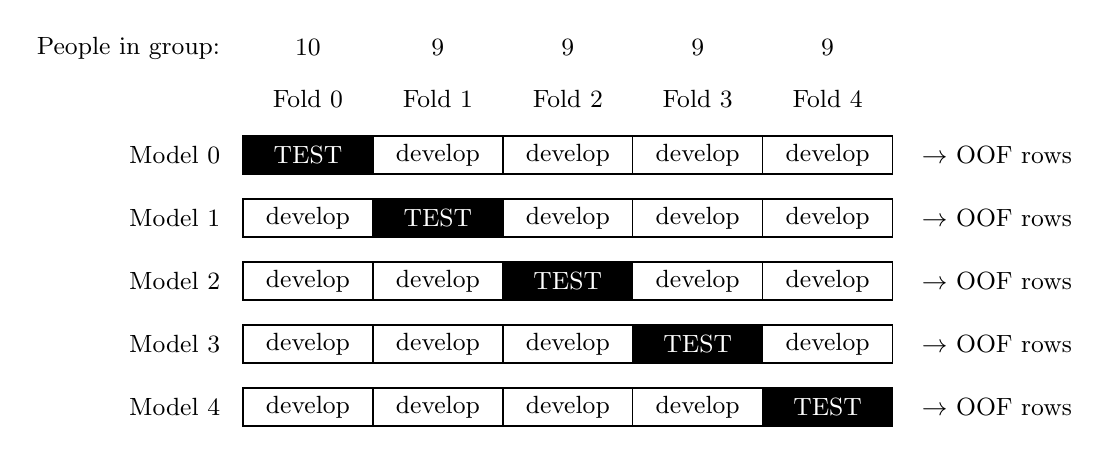
\begin{tikzpicture}[x=1.65cm,y=0.8cm]
\node[anchor=east,font=\small] at (-0.1,1.4) {People in group:};
\foreach \column/\count in {0/10,1/9,2/9,3/9,4/9} {
  \node[font=\small] at (\column+0.5,1.4) {\count};
  \node[font=\small] at (\column+0.5,0.6) {Fold \column};
}
\foreach \row in {0,...,4} {
  \node[anchor=east,font=\small] at (-0.1,-\row-0.3) {Model \row};
  \foreach \column in {0,...,4} {
    \ifnum\row=\column
      \filldraw[fill=black] (\column,-\row) rectangle (\column+1,-\row-0.6);
      \node[text=white,font=\small] at (\column+0.5,-\row-0.3) {TEST};
    \else
      \draw (\column,-\row) rectangle (\column+1,-\row-0.6);
      \node[font=\small] at (\column+0.5,-\row-0.3) {develop};
    \fi
  }
  \node[anchor=west,font=\small] at (5.15,-\row-0.3) {$\rightarrow$ OOF rows};
}
\end{tikzpicture}
\diagramcaption{Each row is a separately trained model. White cells supply
outer-training people, including the inner validation split. The black cell
supplies that model's held-out test people. Fold IDs match the saved files.}
\end{center}

\subsection*{The working policy}
\begin{enumerate}
\item Build one row per speaker and use a stratified five-fold split with seed
42. \emph{Stratified} means keeping both classes represented in every fold.
\item Copy the fold ID to all of that person's sessions, files and windows.
\item Hold one fold aside. Within the remaining people, choose training length
using the inner procedure in Section~\ref{sec:inner}.
\item Refit a fresh model on all outer-training people and predict the held-out
people. The test fold does not choose weights, epochs or the threshold.
\item Save one score per held-out speaker. Repeat for fold IDs 0--4.
\item Join $10+9+9+9+9=46$ speaker rows and calculate the pooled metrics once.
\end{enumerate}

\subsection*{What OOF does and does not mean}
A person may train models for other folds. That is normal. What matters is that
the model used to score that person has never trained on that person's recordings.

OOF is \emph{not} a five-model vote for each of these 46 people. Four of those
five models would have used that person during training. Averaging all five for
the reported OOF score would break the held-out rule.

``Five-fold cross-validation'' names the procedure. ``OOF predictions'' names its
saved held-out outputs. They are two parts of the same evaluation, not competing
methods. OOF also does not make this corpus an independent external test set.

\clearpage
\section{Choose training length without looking at the test fold}\label{sec:inner}
An \key{epoch} is one pass through the selected training windows. Too few epochs
may leave the model undertrained; too many may fit details of the training
people. The project chooses the count using a small validation group taken only
from the outer-training people.

\begin{center}
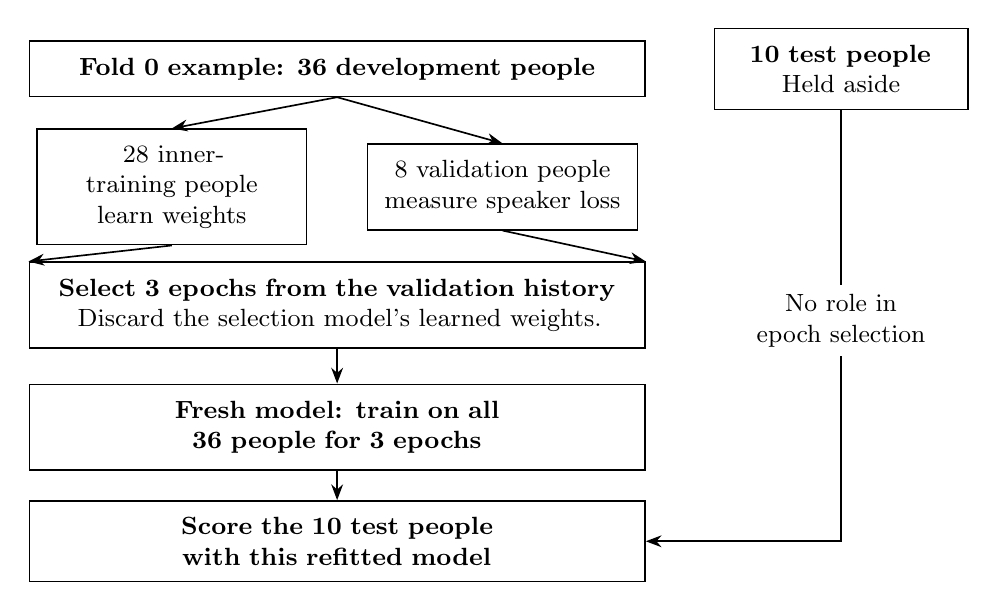
\begin{tikzpicture}[node distance=0.42cm]
\node[box,text width=7.4cm] (dev) at (0,0) {\textbf{Fold 0 example: 36 development people}};
\node[box,text width=2.8cm] (test) at (6.4,0) {\textbf{10 test people}\\Held aside};
\node[box,text width=3.0cm] (fit) at (-2.1,-1.5) {28 inner-training people\\learn weights};
\node[box,text width=3.0cm] (val) at (2.1,-1.5) {8 validation people\\measure speaker loss};
\node[box,text width=7.4cm] (choose) at (0,-3) {\textbf{Select 3 epochs from the validation history}\\Discard the selection model's learned weights.};
\node[box,text width=7.4cm] (refit) at (0,-4.55) {\textbf{Fresh model: train on all 36 people for 3 epochs}};
\node[box,text width=7.4cm] (score) at (0,-6) {\textbf{Score the 10 test people with this refitted model}};
\draw[arrow] (dev.south) -- (fit.north);
\draw[arrow] (dev.south) -- (val.north);
\draw[arrow] (fit.south) -- (choose.north west);
\draw[arrow] (val.south) -- (choose.north east);
\draw[arrow] (choose) -- (refit);
\draw[arrow] (refit) -- (score);
\draw[arrow] (test.south) -- (6.4,-6) -- (score.east);
\node[font=\small,align=center,fill=white] at (6.4,-3.2) {No role in\\epoch selection};
\end{tikzpicture}
\diagramcaption{Actual person counts and selected epoch count for fold 0.
The right-hand path joins only at final testing.}
\end{center}

Inner validation uses a stratified 20\% holdout of the outer-training people.
The selection run allows at most 20 epochs. Its score is the average binary
cross-entropy of \emph{speaker} probabilities, where lower is better. An
improvement must exceed 0.0001; training stops after five epochs without such an
improvement. The best accepted epoch count is then used for a fresh refit.

\begin{center}\small
\begin{tabular}{@{}rrrrrr@{}}
\toprule
Fold & Inner train & Validation & Refit train & Test & Chosen epochs\\
\midrule
\tableinput{generated/training_rows.tex}
\bottomrule
\end{tabular}
\end{center}

Validation people enter the final refit after the epoch count is fixed. Test
people do not. Threshold 0.5 is fixed throughout; it is not chosen from OOF scores.
The split/training seed is $42+\text{fold ID}$ for this inner procedure.

\clearpage
\section{How training learns from the windows}
For each batch, the model produces one logit per window. Binary cross-entropy
compares that output with the known label and penalizes a confident wrong answer.
The optimizer changes the model's weights to reduce the weighted training loss.
Labels are used as targets; they are not appended to the input spectrogram.

\subsection*{Why every window should not have equal influence}
A long recording produces more windows than a short one. A person with two
sessions produces more files than a person with one session. If all windows
were treated equally, those people would have more influence just because more
audio was recorded. The loss weights address this imbalance.

\begin{center}
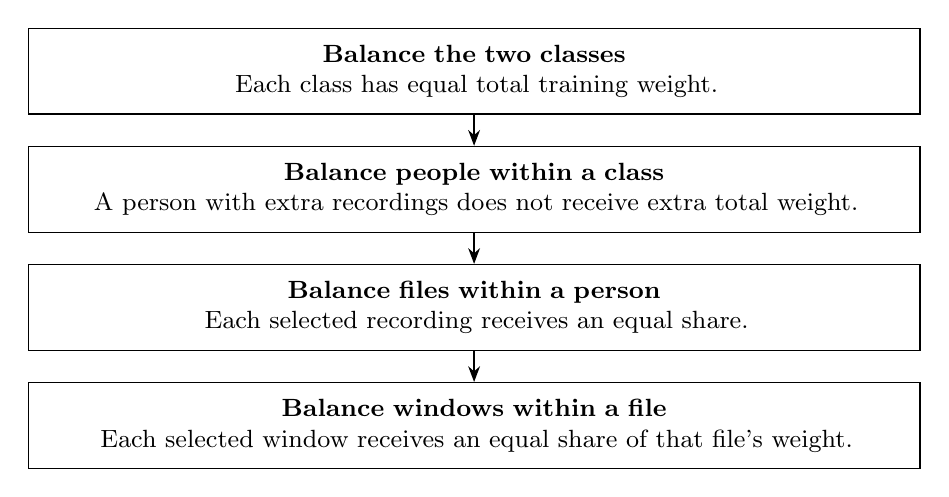
\begin{tikzpicture}
\node[box,text width=10.9cm] (classes) at (0,0) {\textbf{Balance the two classes}\\Each class has equal total training weight.};
\node[box,text width=10.9cm] (people) at (0,-1.5) {\textbf{Balance people within a class}\\A person with extra recordings does not receive extra total weight.};
\node[box,text width=10.9cm] (files) at (0,-3) {\textbf{Balance files within a person}\\Each selected recording receives an equal share.};
\node[box,text width=10.9cm] (windows) at (0,-4.5) {\textbf{Balance windows within a file}\\Each selected window receives an equal share of that file's weight.};
\draw[arrow] (classes) -- (people);
\draw[arrow] (people) -- (files);
\draw[arrow] (files) -- (windows);
\end{tikzpicture}
\diagramcaption{The weight hierarchy for training. Counts are calculated from
the current training partition, not from held-out test people.}
\end{center}

For a window belonging to person $i$, file $j$ and class $c$, its raw weight is
\[
w_{ij}=\frac{1}{N_c\,F_i\,W_{ij}},
\]
where $N_c$ is the number of training people in class $c$, $F_i$ is that person's
number of training files, and $W_{ij}$ is the number of selected windows in that
file. All weights are then rescaled so their average is 1. This keeps their
relative importance while keeping the overall loss scale convenient.

\begin{center}
\begin{tabularx}{\linewidth}{@{}L{3.7cm}L{2.5cm}Y@{}}
\toprule
Setting & Value & What it means\\
\midrule
Optimizer & AdamW & Updates weights using the training loss.\\
Learning rate & 0.001 & Sets the scale of an update.\\
Weight decay & 0.0001 & Discourages unnecessarily large weights.\\
Batch size & 16 windows & Number of windows processed in one batch.\\
Dropout & 0.2 & Randomly drops selected activations during training.\\
Gradient norm limit & 1.0 & Limits unusually large update signals.\\
Compute & CPU, 4 threads & The completed run used deterministic Torch settings.\\
\bottomrule
\end{tabularx}
\end{center}

During prediction the model is in evaluation mode: dropout is off, and no weights
are updated. The saved checkpoint is the refitted model, not the discarded
inner-selection model.

\clearpage
\section{From window scores to one speaker decision}
The model first scores short windows, but the study's question is about people.
The pipeline therefore averages twice: first within a recording, then across
that person's recordings. It averages probabilities, not hard yes/no votes.

\begin{center}
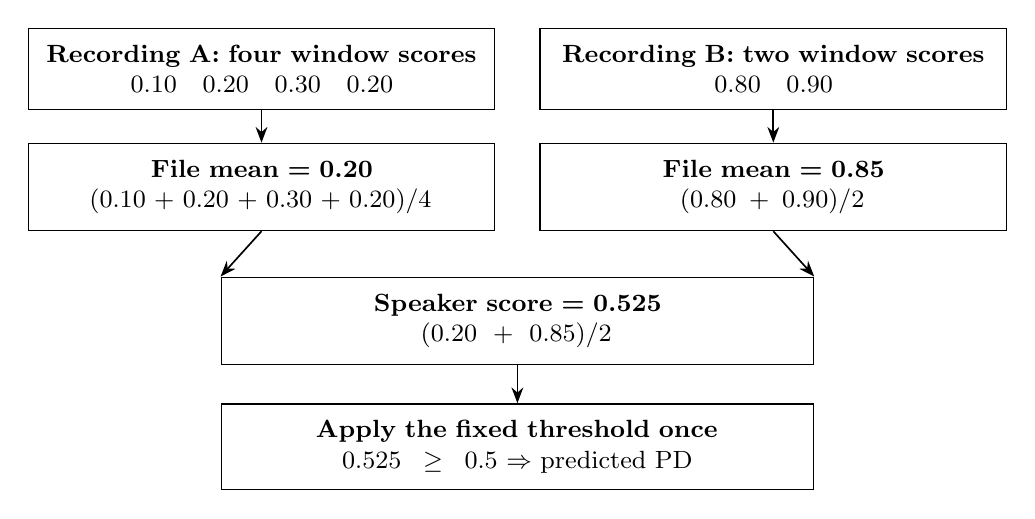
\begin{tikzpicture}
\node[box,text width=5.5cm] (a) at (0,0) {\textbf{Recording A: four window scores}\\0.10\quad0.20\quad0.30\quad0.20};
\node[box,text width=5.5cm] (b) at (6.5,0) {\textbf{Recording B: two window scores}\\0.80\quad0.90};
\node[box,text width=5.5cm] (am) at (0,-1.5) {\textbf{File mean = 0.20}\\$(0.10+0.20+0.30+0.20)/4$};
\node[box,text width=5.5cm] (bm) at (6.5,-1.5) {\textbf{File mean = 0.85}\\$(0.80+0.90)/2$};
\node[box,text width=7.1cm] (person) at (3.25,-3.2) {\textbf{Speaker score = 0.525}\\$(0.20+0.85)/2$};
\node[box,text width=7.1cm] (decision) at (3.25,-4.8) {\textbf{Apply the fixed threshold once}\\$0.525\geq0.5$ $\Rightarrow$ predicted PD};
\draw[arrow] (a) -- (am);
\draw[arrow] (b) -- (bm);
\draw[arrow] (am.south) -- (person.north west);
\draw[arrow] (bm.south) -- (person.north east);
\draw[arrow] (person) -- (decision);
\end{tikzpicture}
\diagramcaption{A made-up example to explain the arithmetic, not a real
participant. Both files have equal influence on the final speaker score.}
\end{center}

If all six windows in this example were averaged directly, the answer would be
$2.50/6\approx0.417$. Recording A would count twice as much because it supplied
twice as many windows. The two-stage average avoids that particular imbalance.

For a person with $F_i$ files and $W_{ij}$ windows in file $j$, the rule is
\[
\bar p_{ij}=\frac{1}{W_{ij}}\sum_{k=1}^{W_{ij}}p_{ijk},
\qquad
p_i=\frac{1}{F_i}\sum_{j=1}^{F_i}\bar p_{ij}.
\]
Here $p_{ijk}$ is a window score, $\bar p_{ij}$ is a file score, and $p_i$ is the
speaker score. Prediction is 1 when $p_i\geq0.5$, otherwise 0.

\subsection*{Why this still needs careful interpretation}
Files have equal weight, but task families do not necessarily have equal weight:
a person with many vowel recordings gives that family more file slots. The
main cohort also contains 10--32 recordings per person, median 16. Averaging
can reduce random noise, but it can preserve a recording signature that appears
across all of a person's files.

\rulebox{\textbf{One person, one row, one decision.} The final table records
speaker ID, true label, probability, threshold, prediction, fold and sheet flag.
Only these speaker rows enter the headline metrics.}

\clearpage
\section{Every fold, followed by the pooled result}\label{sec:results}
These are the main saved results for \key{v2.0 / Arannamoy PatchTST / main}.
All five metrics are percentages. Fold IDs are 0--4, exactly as stored in the run.
Each row evaluates only the people held out from that row's model.

\begin{center}\small
\setlength{\tabcolsep}{4.5pt}
\begin{tabular}{@{}lrrrrrr@{}}
\toprule
Fold & People & F1 & Recall & Specificity & Precision & Accuracy\\
\midrule
\tableinput{generated/fold_rows.tex}
\bottomrule
\end{tabular}
\captionof{table}{Held-out fold results and their mean $\pm$ sample standard
deviation. SD describes variation across these five folds, not uncertainty in
a new clinical population.}
\end{center}

\subsection*{Pooled result: calculate once from all 46 held-out people}
\begin{center}
\begin{tabular}{@{}rrrrrr@{}}
\toprule
People & F1 & Recall & Specificity & Precision & Accuracy\\
\midrule
\tableinput{generated/pooled_row.tex}
\bottomrule
\end{tabular}
\end{center}

\begin{center}
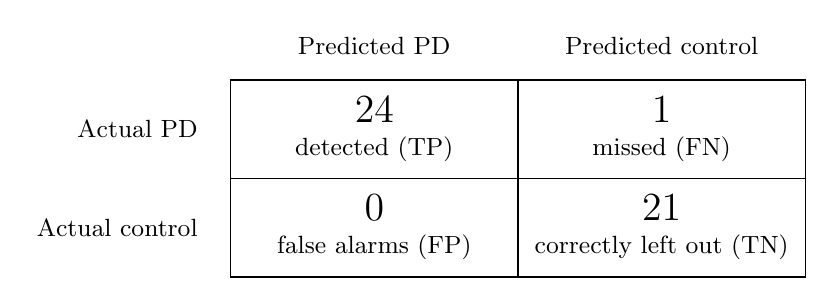
\begin{tikzpicture}[x=3.65cm,y=1.25cm]
\node[font=\small] at (0.5,0.35) {Predicted PD};
\node[font=\small] at (1.5,0.35) {Predicted control};
\draw (0,0) rectangle (2,-2);
\draw (1,0) -- (1,-2);
\draw (0,-1) -- (2,-1);
\node[anchor=east,font=\small] at (-0.08,-0.5) {Actual PD};
\node[anchor=east,font=\small] at (-0.08,-1.5) {Actual control};
\node[align=center] at (0.5,-0.5) {\Large 24\\\small detected (TP)};
\node[align=center] at (1.5,-0.5) {\Large 1\\\small missed (FN)};
\node[align=center] at (0.5,-1.5) {\Large 0\\\small false alarms (FP)};
\node[align=center] at (1.5,-1.5) {\Large 21\\\small correctly left out (TN)};
\end{tikzpicture}
\diagramcaption{The pooled confusion matrix: 25 patients and 21 controls.}
\end{center}

\key{Why pooled F1 is not the mean fold F1.} Pooling first adds the confusion
counts: $TP=24$, $FN=1$, $TN=21$, $FP=0$. Then
\[
\mathrm{F1}=\frac{2TP}{2TP+FP+FN}=\frac{48}{49}=97.96\%,
\quad
\mathrm{Accuracy}=\frac{24+21}{46}=97.83\%.
\]
The mean fold F1 is 97.78\%, because it averages five percentages instead.
Both are useful; the pooled five-metric result is the primary result.

\key{The one error.} Fold 4 misses one patient at speaker probability 0.4159119,
below the fixed 0.5 threshold. That fold detects four of its five patients and
correctly classifies all four controls. No threshold is changed after seeing
this error.

\clearpage
\section{Reading the speaker scores and the five metrics}
Figure~\ref{fig:probabilities} plots the actual saved OOF probabilities. No model
is trained to draw it. The horizontal dashed line is the same 0.5 threshold used
for every fold.

\begin{center}
\begin{tikzpicture}
\begin{axis}[
width=14.6cm,height=7.0cm,
xmin=0,xmax=47,ymin=-0.04,ymax=1.04,
xtick={1,10,21,30,40,46},ytick={0,0.25,0.5,0.75,1},
xlabel={Speaker display order (46 people)},ylabel={OOF model score},
axis lines=left,tick label style={font=\small},label style={font=\small},
legend style={font=\small,draw=black,fill=white,at={(0.5,1.03)},anchor=south,legend columns=2},
clip=false]
\addplot[only marks,mark=o,mark size=2.1pt,black,mark options={fill=white}] table[x=speaker_order,y=probability,col sep=comma]{generated/controls.csv};
\addlegendentry{Elderly control}
\addplot[only marks,mark=*,mark size=2.1pt,black] table[x=speaker_order,y=probability,col sep=comma]{generated/patients.csv};
\addlegendentry{PD}
\addplot[black,dashed,forget plot] coordinates {(0,0.5) (47,0.5)};
\draw[densely dotted] (axis cs:21.5,0) -- (axis cs:21.5,1);
\node[font=\small,anchor=west,fill=white] at (axis cs:2,0.54) {decision threshold};
\node[font=\small,anchor=west,fill=white] at (axis cs:24,0.32) {one missed patient};
\draw[arrow] (axis cs:24,0.34) -- (axis cs:22,0.4159119);
\end{axis}
\end{tikzpicture}
\diagramcaption{Actual main-cohort scores. Open circles are controls; filled
circles are patients. For display only, people are grouped by true class and
ordered by score within each group. This ordering is not a training input.
One filled circle falls below the decision threshold.}\label{fig:probabilities}
\end{center}

\begin{center}\small
\begin{tabularx}{\linewidth}{@{}L{2.1cm}L{3.6cm}Y@{}}
\toprule
Metric & Formula & Question it answers\\
\midrule
F1 & $2TP/(2TP+FP+FN)$ & How well are precision and recall balanced?\\
Recall & $TP/(TP+FN)$ & Of the patients, how many were detected?\\
Specificity & $TN/(TN+FP)$ & Of the controls, how many were correctly classified?\\
Precision & $TP/(TP+FP)$ & Of the people predicted as PD, how many were PD here?\\
Accuracy & $(TP+TN)/N$ & Of all people, how many were classified correctly?\\
\bottomrule
\end{tabularx}
\end{center}

F1 leaves out true negatives, so it cannot replace specificity. Accuracy can
hide missed patients, so it cannot replace recall. Reporting the five together
shows the different types of success and error.

Precision depends on how common PD is in the evaluated group. This sample is
close to half patients; its precision is not the positive predictive value of
screening a general community. The probability axis likewise shows model output,
not proven clinical risk.

The sample is small. One extra missed patient changes recall by four percentage
points; one extra false alarm changes specificity by about 4.76 points. The five
fold models also share much of their training data. Fold variation should not
be read as five independent clinical trials.

\clearpage
\section{Data leakage: the routes and the controls}\label{sec:leakage}
\key{Data leakage} means that information from the held-out evaluation enters
learning or model selection in a way it should not. A high score can then reflect
prior exposure rather than a fair prediction on an unseen person.

\begin{center}
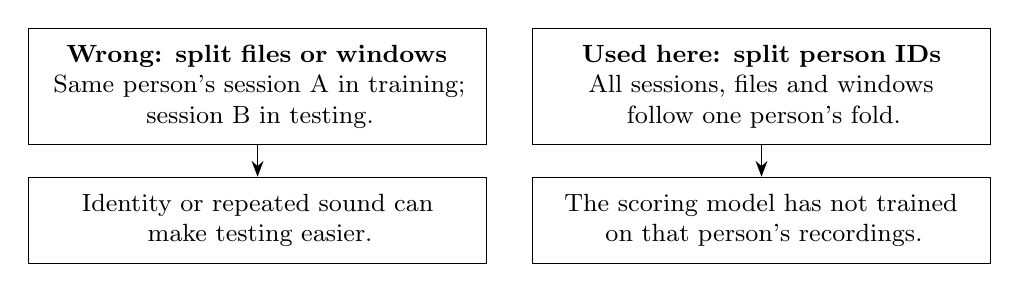
\begin{tikzpicture}
\node[box,text width=5.4cm] (bad) at (0,0) {\textbf{Wrong: split files or windows}\\Same person's session A in training;\\session B in testing.};
\node[box,text width=5.4cm] (good) at (6.4,0) {\textbf{Used here: split person IDs}\\All sessions, files and windows\\follow one person's fold.};
\node[box,text width=5.4cm] (badeffect) at (0,-1.7) {Identity or repeated sound can\\make testing easier.};
\node[box,text width=5.4cm] (goodeffect) at (6.4,-1.7) {The scoring model has not trained\\on that person's recordings.};
\draw[arrow] (bad) -- (badeffect);
\draw[arrow] (good) -- (goodeffect);
\end{tikzpicture}
\diagramcaption{Why the split must follow people. Speaker separation addresses
identity overlap; it does not automatically address all recording differences.}
\end{center}

\begin{center}\small
\begin{tabularx}{\linewidth}{@{}L{3.4cm}Y@{}}
\toprule
Possible route & What the pipeline does about it\\
\midrule
Same person in train and test & Link known repeat sessions before splitting;
check disjoint speaker IDs in outer and inner splits.\\
Overlapping audio windows & Create windows within already assigned speaker groups;
never randomly divide windows across train and test.\\
Identical audio under another ID & Compare raw-file and decoded-audio hashes;
no identical decoded signal was found across the 773 main files under different people.\\
Test set chooses training length & Choose epochs on inner validation speakers;
refit before the held-out fold is scored.\\
Test set chooses the threshold & Fix the threshold at 0.5 for all folds.\\
Preprocessing learns from test people & Use fixed per-recording audio transforms
and fixed model scaling; there is no cohort-fitted normalizer in this PatchTST.\\
Metadata reveals the answer & Keep IDs, labels, dates, age, sex and rate out of
the feature tensor. Labels enter the training loss only.\\
Wrong or stale feature cache & Cache names use the audio bytes' hash and feature
settings. Check shape and finite values; the audit recomputed all main features.\\
Repeated tuning on reported results & Record earlier development and freeze the
current protocol. This history cannot be undone by rerunning the same folds.\\
\bottomrule
\end{tabularx}
\end{center}

\key{Why caching every file is allowed here.} A fixed transform can process a
held-out file without learning from it, just as a saved model must eventually
read a test input. If future preprocessing learns a mean, feature selection or
any other parameter from multiple people, that learning must occur inside the
training partition and then be applied unchanged to its held-out partition.

\key{Remaining distinction.} Recording-condition confounding can survive every
identity check. Different people can still share class-related microphone or
room cues. Section~\ref{sec:checks} explains the evidence for that concern.

\clearpage
\section{What the extra checks tell us about this same model}\label{sec:checks}
The project keeps one primary model and the main pooled result. Two checks of
the same model ask whether conclusions depend on flagged controls or on files
originally recorded at another sample rate.

\begin{center}\footnotesize
\setlength{\tabcolsep}{3.7pt}
\begin{tabular}{@{}lrrrrrr@{}}
\toprule
Evaluation & People & F1 & Recall & Specificity & Precision & Accuracy\\
\midrule
\tableinput{generated/sensitivity_rows.tex}
\bottomrule
\end{tabular}
\captionof{table}{Three views of the same PatchTST procedure, all at speaker
level. These are checks on the primary result, not three competing models.}
\end{center}

\key{Flag exclusion} removes the three flagged controls from the main OOF table.
It does not retrain the model. \key{Native-rate retraining} removes every file
originally sampled at 44.1 kHz before both training and evaluation, leaving 39
people and 613 files. It retains the existing person-fold assignments.

The sole patient missed in the main run is among the seven people removed by
native-rate filtering. The main predictions are already perfect on the retained
39 people. The native-only retraining is real, but its perfect result is not
independent confirmation or a controlled improvement on an unchanged cohort.

\subsection*{The remaining recording-condition problem}
\begin{center}
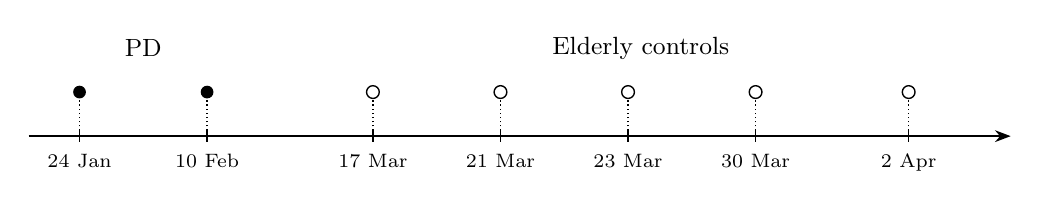
\begin{tikzpicture}[x=1.62cm,y=0.7cm]
\draw[arrow] (0,0) -- (7.7,0);
\foreach \x/\lab in {0.4/24 Jan,1.4/10 Feb,2.7/17 Mar,3.7/21 Mar,4.7/23 Mar,5.7/30 Mar,6.9/2 Apr} {
  \draw (\x,0.1) -- (\x,-0.1);
  \node[below,font=\scriptsize] at (\x,-0.14) {\lab};
}
\foreach \x in {0.4,1.4} {
  \fill (\x,0.8) circle (2.3pt);
  \draw[densely dotted] (\x,0.1) -- (\x,0.7);
}
\foreach \x in {2.7,3.7,4.7,5.7,6.9} {
  \draw[fill=white] (\x,0.8) circle (2.3pt);
  \draw[densely dotted] (\x,0.1) -- (\x,0.7);
}
\node[font=\small] at (0.9,1.6) {PD};
\node[font=\small] at (4.8,1.6) {Elderly controls};
\end{tikzpicture}
\diagramcaption{Native-16-kHz recording dates in 2017, ordered rather than
drawn to a true time scale. Filled points are PD dates; open points are control
dates. Every date has only one class.}
\end{center}

All five native-rate speaker folds share dates between training and testing.
Dates are not network inputs, but gain, microphone or room differences could
be audible. Quietest-frame digital levels differ strongly between the groups;
these frames have not been verified as speech-free silence.

The saved main decisions also survive shuffling frames or replacing each
window with its repeated average spectrum. This means those decisions do not
require the original within-window temporal detail. It does not establish that
all signal is noise, or that temporal information is never useful.

\key{How to address the remaining problem.} Predeclare gain/channel/noise stress
tests; verify what low-energy segments contain; and later evaluate recordings
with patients and controls collected under matched conditions. Only two native
PD dates exist, so five two-class, date-disjoint test folds cannot be created.
External benchmarking remains the next project phase.

\clearpage
\section{Reproducibility: connect every number to a saved file}
The official trained result is v2.0. The active readable implementation is called
v2.1; that code rewrite is not a new trained result. Report version 1.0 is a
document version, separate from either experiment or code version.

\subsection*{The frozen result directory}
\sourcepath{artifacts/runs/20261012T183328Z_f-all_cead14cc32f1/}

\begin{center}\small
\begin{tabularx}{\linewidth}{@{}L{7.7cm}Y@{}}
\toprule
File relative to that run & What it records\\
\midrule
\path{config.yaml} & Exact settings used by the completed run.\\
\path{protocol.json}, \path{folds.csv} & Cohort, source fingerprints and speaker assignments.\\
\path{source/} & Archived implementation and dependency files.\\
\path{main/arannamoy/manifest.csv} & The 773 input recordings and their metadata.\\
\path{main/arannamoy/fold_0/split.json} & Training, validation and test person IDs for fold 0.\\
\path{main/arannamoy/fold_0/selection.json} & Chosen epoch count and model size.\\
\path{main/arannamoy/fold_0/checkpoint.pt} & The refitted model's learned weights.\\
\path{main/arannamoy/speaker_predictions.csv} & The 46 pooled OOF speaker rows.\\
\path{main/arannamoy/metrics.json} & Pooled metrics, fold metrics and their spread.\\
\bottomrule
\end{tabularx}
\end{center}

The same per-fold files exist for fold IDs 1--4. Each training run stores an
inner-selection history and a refit history. File hashes are fingerprints of
file contents; they help detect accidental changes but do not establish that a
scientific interpretation is correct.

\subsection*{What the latest audit actually reproduced}
Audit v2.0-audit.2 recomputed all 773 main log-mel arrays from raw audio. With one
BLAS arithmetic thread, all arrays matched the cache bit for bit. All ten
PatchTST checkpoints, five main and five native-only, reproduced their saved
decisions using freshly extracted inputs. A tiny initial discrepancy of about
$1.5\times10^{-5}$ dB was traced to arithmetic thread count. The initial failure
and its resolution are both retained.

This is a raw-input and prediction replay check, not a full new training run.
It confirms that the saved model, inputs and reported outputs agree. It does
not remove recording-condition confounding.

\subsection*{How to make a new run}
From the project root, prepare a fresh run, then replace \texttt{NEW\_RUN} below
with the directory printed by the preparation command:
{\small
\begin{verbatim}
uv sync --locked
uv run python scripts/compare_members.py --prepare
uv run python scripts/compare_members.py --run NEW_RUN --member arannamoy
\end{verbatim}
}
The last command runs this member's main and native-rate scenarios. A v2.1 run
gets its own results; it is not the completed v2.0 experiment. Historical
checkpoints load through \texttt{PatchTST.load\_v2\_checkpoint}.

\clearpage
\section{Key terms and the final interpretation}
\begin{center}
\begin{tabularx}{\linewidth}{@{}L{3.0cm}Y@{}}
\toprule
Term & Meaning in this project\\
\midrule
Speaker & One person, even if that person has several sessions or folders.\\
Recording & One WAV file from one speech task.\\
Native sample rate & Samples per second in the original WAV, before conversion.\\
Frame & One short frequency-energy measurement, taken every 10 ms.\\
Mel band & A frequency range used to summarize sound energy.\\
Log-mel & Mel-band power expressed on a fixed logarithmic scale.\\
Window & The 400-frame input given to the model at one time.\\
Patch & A 16-frame piece of one band inside that window.\\
Parameter & A number the model learns during training.\\
Epoch & One pass through the selected training windows.\\
Validation & Training-side people used to choose how long to train.\\
Test fold & People excluded from the model used to predict them.\\
OOF prediction & A score made by the model trained without that person's fold.\\
Pooled result & Metrics recalculated after joining all held-out speaker rows.\\
Leakage & Held-out information improperly entering fitting or selection.\\
Confounding & Another group-related difference can help explain the score.\\
Checkpoint & A saved copy of the model's learned weights.\\
\bottomrule
\end{tabularx}
\end{center}

\subsection*{What is established}
The pipeline consistently converts audio into the stated input, keeps known
repeat sessions together, chooses epochs inside training people, and reports
one held-out decision per speaker. The main saved result is 24 detected patients,
one missed patient, 21 correctly classified controls and no false alarms.
The published tables in this report are generated from saved speaker scores.

\subsection*{What is not established}
The small, repeatedly studied corpus does not establish performance in a new
clinic. Keeping people separate does not make recording conditions identical.
The high score does not show that temporal attention is necessary, and the
perfect native-rate check is not an independent replication. These limits are
part of the result's meaning, not a reason to hide the result.

\subsection*{The main lesson}
\rulebox{A trustworthy speech-classification report must explain \emph{who was
held out}, \emph{what the model could see}, and \emph{how the final person-level
decision was made}. A high percentage alone does not answer those questions.}

\clearpage
\begin{thebibliography}{9}
\addcontentsline{toc}{section}{References}
\bibitem{dataport}
G. Dimauro and F. Girardi. \emph{Italian Parkinson's Voice and Speech}.
IEEE DataPort, 2019. DOI: \href{https://doi.org/10.21227/aw6b-tg17}{10.21227/aw6b-tg17}.

\bibitem{voxtester}
G. Dimauro et al. ``VoxTester, software for digital evaluation of speech changes
in Parkinson disease.'' \emph{IEEE International Symposium on Medical
Measurements and Applications (MeMeA)}, 2016.
DOI: \href{https://doi.org/10.1109/MeMeA.2016.7533761}{10.1109/MeMeA.2016.7533761}.

\bibitem{access}
G. Dimauro, V. Di Nicola, V. Bevilacqua, D. Caivano and F. Girardi.
``Assessment of Speech Intelligibility in Parkinson's Disease Using a
Speech-To-Text System.'' \emph{IEEE Access}, vol. 5, pp. 22199--22208, 2017.
DOI: \href{https://doi.org/10.1109/ACCESS.2017.2762475}{10.1109/ACCESS.2017.2762475}.

\bibitem{patchtst}
Y. Nie, N. H. Nguyen, P. Sinthong and J. Kalagnanam.
``A Time Series is Worth 64 Words: Long-term Forecasting with Transformers.''
\emph{ICLR}, 2023. \href{https://arxiv.org/abs/2211.14730}{arXiv:2211.14730}.

\bibitem{generalization}
M. Hire\v{s}, P. Drot\'ar, N. D. Pah, Q. C. Ngo and D. K. Kumar.
``On the inter-dataset generalization of machine learning approaches to
Parkinson's disease detection from voice.'' \emph{International Journal of
Medical Informatics}, vol. 179, 105237, 2023.
DOI: \href{https://doi.org/10.1016/j.ijmedinf.2023.105237}{10.1016/j.ijmedinf.2023.105237}.

\bibitem{internal}
A. Mondal. Project evidence, experiment v2.0 and audits v2.0-audit.1--2, 2026.
The frozen data and code provenance is identified in Section 16.
Supporting project documents:\\
\sourcepath{docs/corrected_comparison.md}\\
\sourcepath{docs/corrected_results.md}\\
\sourcepath{docs/high_score_audit.md}\\
\sourcepath{docs/publication_readiness_audit.md}
\end{thebibliography}

\subsection*{Evidence and build notes}
The exact model settings come from the frozen run's configuration, not from
a later edit to the active configuration. Fold metrics, selected epochs and
speaker probabilities are read from saved artifacts. No training takes place
when this report is built.

The complete audit record for the raw-audio recheck is under:\\
\sourcepath{artifacts/runs/20261012T215648Z_v2.0-audit.2_2167119cc167/}

The report source and build instructions are under:\\
\sourcepath{docs/whitepaper_v1_0/}

\subsection*{Document and figures}
This report uses a restrained, single-column whitepaper layout with serif text,
black rules, equations and diagrams. The speaker-score plot uses actual saved
predictions. The worked averaging example and input-shape sketches are
illustrative. The PDF, source and build manifest are supplied together so the
report can be checked and updated.

This report describes an internal, revised evaluation after prior development
on the same corpus. Broader cross-dataset concerns are discussed in
Hire\v{s} et al.~\cite{generalization}. The next benchmark phase should use a
frozen procedure and clearly state which data were available during development.

\end{document}
